\documentclass[12pt,a4paper,utf8]{ctexart}
\usepackage{graphicx}
\usepackage{amsmath}
\usepackage{amssymb}
\usepackage{subfig}
\usepackage{cite}
\usepackage[ntheorem]{empheq}
\usepackage{enumitem}
\usepackage{fullpage}
\usepackage{cleveref}
\usepackage{cellspace}
\usepackage{listings}
\usepackage{color}
\definecolor{gray}{rgb}{0.5,0.5,0.5}
\definecolor{dkgreen}{rgb}{.068,.578,.068}
\definecolor{dkpurple}{rgb}{.320,.064,.680}

% set Matlab styles
\lstset{
   language=Matlab,
   keywords={break,case,catch,continue,else,elseif,end,for,function,
      global,if,otherwise,persistent,return,switch,try,while},
   basicstyle=\ttfamily,
   keywordstyle=\color{blue}\bfseries,
   commentstyle=\color{dkgreen},
   stringstyle=\color{dkpurple},
   backgroundcolor=\color{white},
   tabsize=4,
   showspaces=false,
   showstringspaces=false
}

\begin{document}
\CJKfamily{zhkai}	

\begin{center}
\textbf{作业一}\\
\textbf{姓名 ~何春望~ 学号 ~PB17000075~ 日期 ~2020.10.17}\\
\end{center}
\textit{}
\vspace{\baselineskip}

\begin{enumerate}
\item[第一题] \textbf{重心插值公式(barycentric interpolation formula)}  
\subitem(a)
\subsubitem(1)
易知
\begin{equation}
   \begin{aligned}
      \ell_{j}\left(x_{k}\right)&=\frac{\ell\left(x_{k}\right)}{\ell^{'}(x_j)(x_k-x_j)}\\
      &=\frac{\prod\limits_{i=0}^n (x_k-x_i)}{\prod\limits_{i \neq j} (x_j-x_i) \cdot (x_k-x_j)}\\
      &=\left\{\begin{array}{rr}
         \frac{0}{\prod\limits_{i \neq j} (x_j-x_i) \cdot (x_k-x_j)} = 0 & k \neq j \\
         \frac{\prod\limits_{i \neq j} (x_k-x_i)}{\prod\limits_{i \neq j} (x_j-x_i)} = 1 & k = j
      \end{array}\right.
   \end{aligned}
\end{equation}

即$\ell_j(x)=\frac{\ell(x)}{\ell^{'}(x_j)(x-x_j)}$可以作为Lagrange基函数.

\subsubitem(2)
\begin{equation}
   \begin{aligned}
      p(x) &= \sum_{j = 0}^n \ell_j(x)f_j\\
      &= \ell(x) \sum_{j = 0}^n \frac{1}{\ell^{'}(x_j)} \cdot \frac{f_j}{x - x_j}
   \end{aligned}
\end{equation}

令$\lambda_j=\frac{1}{\ell^{'}(x_j)}$,即得
\begin{equation}
   p(x) = \ell(x) \sum_{j = 0}^n \frac{\lambda_j}{x - x_j} f_j
\end{equation}

\subitem(b)
\subsubitem(1)
取$f(x) \equiv 1$,
\begin{equation}
   f(x)=p(x)+R(x)=\sum_{j=0}^n f(j)\ell_j(x) + \frac{f^{(n+1)}(\xi)}{(n+1)!} \prod_{k=0}^n (x-x_k)
\end{equation}
代入$f(j) = 1$,$f^{(n+1)}(x) = 0$,得
\begin{equation}
   \sum_{j = 0}^n \ell_j(x) = 1
\end{equation}

\subsubitem(2)
由上式(5),
\begin{equation}
   1 = \sum_{j = 0}^n \ell_j(x) = \sum_{j = 0}^n \frac{\ell(x)}{\ell^{'}(x_j)(x-x_j)}
\end{equation}
故$\ell(x) = {1} / {\sum_{j = 0}^n \frac{1}{\ell^{'}(x_j)(x-x_j)}} = {1} / {\sum_{j = 0}^n \frac{\lambda_j}{x - x_j}}$,
代入(3)即得
\begin{equation}
   \begin{aligned}
      p(x) &= \ell(x) \sum_{j = 0}^n \frac{\lambda_j}{x - x_j} f_j\\
      &= \frac{\sum_{j = 0}^n\limits \frac{\lambda_j f_j}{x - x_j}}{\sum_{j = 0}^n\limits \frac{\lambda_j}{x - x_j}}
   \end{aligned}
\end{equation}

\subitem(c)
先证明$\prod\limits_{k=1}^{n-1}\sin\frac{k\pi}{n}=\frac{n}{2^{n-1}}$:\\
设$\epsilon=\cos\frac{\pi}{n}+i\sin\frac{\pi}{n}$($i$为虚数单位),则$1,\epsilon,\epsilon^2,\ldots,\epsilon^{2(n-1)}$
为$x^{2n}-1=0$的根,且
\begin{equation}
   \sin\frac{k\pi}{n}=\frac{\epsilon^k-\epsilon^{-k}}{2i}=\frac{\epsilon^{2k}-1}{2i\epsilon^k},
\end{equation}
所以
\begin{equation}
   \begin{aligned}
      {}&\prod_{k=1}^{n-1}\sin\frac{k\pi}{n}\\
      =&\frac{(\epsilon^{2}-1) (\epsilon^{4}-1) \ldots [\epsilon^{2(n-1)}-1]}{2^{n-1}i^{n-1}\epsilon^{\frac{1}{2} n(n-1)}}\\
      =&\frac{(-1)^{n-1}(\epsilon^2-1)(\epsilon^4-1)\ldots[\epsilon^{2(n-1)}-1]}{2^{n-1}(i^{n-1})^2}\\
      =&\frac{(1-\epsilon^2)(1-\epsilon^4)\ldots[1-\epsilon^{2(n-1)}]}{2^{n-1}},
   \end{aligned}
\end{equation}
又因为
\begin{equation}
   (x^2-\epsilon^2)(x^2-\epsilon^4)\ldots[x^2-\epsilon^{2(n-1)}]=x^{2(n-1)}+x^{2(n-2)}+\ldots+x^{2}+1,
\end{equation}
所以
\begin{equation}
   (1-\epsilon^2)(1-\epsilon^4)\ldots[1-\epsilon^{2(n-1)}]=n,	
\end{equation}
因此,
\begin{equation}
   \prod_{k=1}^{n-1}\sin\frac{k\pi}{n}=\frac{n}{2^{n-1}}.
\end{equation}
下面化简插值权重:
\begin{equation}
   \lambda_j=\frac{1}{\ell^{'}(x_j)}
\end{equation}
而
\begin{equation}
   \begin{aligned}
      \ell^{'}(x_j)&=\prod_{k\ne j}(x_j-x_k)\\
      &=\prod_{k \ne j}(\cos\frac{j\pi}{n}-\cos\frac{k\pi}{n})\\
      &=\prod_{k \ne j}-2\sin\frac{(j+k)\pi}{2n}\sin\frac{(j-k)\pi}{2n}\\
      &=(-2)^n\prod_{k \ne j}\sin\frac{(j+k)\pi}{2n}\sin\frac{(j-k)\pi}{2n}
   \end{aligned}
\end{equation}

当$j=0$时,
\begin{equation}
   \begin{aligned}
      \ell^{'}(x_0)&=(-2)^n\prod_{k=1}^n\sin\frac{k\pi}{2n}\sin\frac{-k\pi}{2n}\\
      &=2^n\prod_{k=1}^n\sin\frac{k\pi}{2n}\sin\frac{k\pi}{2n}\\
      &=2^n(\sin\frac{\pi}{2})^2\prod_{k=1}^{n-1}\sin\frac{k\pi}{2n}\sin\frac{k\pi}{2n}\\
      &=2^n\prod_{k=1}^{n-1}\sin\frac{k\pi}{2n}\sin\frac{k\pi}{2n}\\
      &=2^n\prod_{k=1}^{n-1}\sin\frac{k\pi}{2n}\sin\frac{(2n-k)\pi}{2n}\\
      &=2^n\sin\frac{n\pi}{2n}\prod_{k=1}^{n-1}\sin\frac{k\pi}{2n}\prod_{k=n+1}^{2n-1}\sin\frac{k\pi}{2n}\\
      &=2^n\prod_{k=1}^{2n-1}\sin\frac{k\pi}{2n}
   \end{aligned}
\end{equation}
由于$\prod\limits_{k=1}^{n-1}\sin\frac{k\pi}{n}=\frac{n}{2^{n-1}}$,
所以$\prod\limits_{k=1}^{2n-1}\sin\frac{k\pi}{2n}=\frac{2n}{2^{2n-1}}=\frac{n}{2^{2n-2}}$,\\
由推导过程可得,$\prod_{k=1}^n(\sin\frac{k\pi}{2n})^2=\frac{n}{2^{2n-2}}$.\\
\begin{equation}
   \begin{aligned}
      \ell^{'}(x_0)&=2^n\prod_{k=1}^{2n-1}\sin\frac{k\pi}{2n}\\
      &=2^n\frac{n}{2^{2n-2}}\\
      &=\frac{n}{2^(n-2)}
   \end{aligned}
\end{equation}
故$\lambda_0=\frac{1}{\ell^{'}(x_0)}=\frac{2^{(n-2)}}{n}$\\

当$j=n$时,
\begin{equation}
   \begin{aligned}
      \ell^{'}(x_n)&=(-2)^n\prod_{k=0}^{n-1}\sin\frac{(n+k)\pi}{2n}\sin\frac{{n-k}\pi}{2n}\\
      &=(-2)^n \prod_{k=n}^{2n-1}\sin\frac{k\pi}{2n} \prod_{k=1}^{n}\sin\frac{k\pi}{2n}\\
      &=(-2)^n \prod_{k=1}^{2n-1}\sin\frac{k\pi}{2n}\\
      &=(-2)^n \frac{n}{2^{2n-2}}\\
      &=(-1)^n \frac{n}{2^{n-2}}
   \end{aligned}
\end{equation}
故$\lambda_n = \frac{1}{\ell^{'}(x_n)} = \frac{2^(n-2)}{n}(-1)^n$

当$1 \le j \le n-1$时,
\begin{equation}
   \begin{aligned}
      \ell^{'}(x_j)&=(-2)^n \prod_{k\ne j} \sin\frac{(j+k)\pi}{2n} \sin\frac{(j-k)\pi}{2n}\\
      &=(-2)^n \cdot \prod_{k=j}^{2j-1} \sin\frac{k\pi}{2n} \prod_{k=2j+1}^{n+j} \sin\frac{k\pi}{2n} \prod_{k=j-n}^{-1} \sin\frac{k\pi}{2n} \prod_{k=1}^{j} \sin\frac{k\pi}{2n}\\
      &=(-2)^n \cdot (-1)^{n-j} \prod_{k=j}^{2j-1}\sin\frac{k\pi}{2n} \prod_{k=2j+1}^{n+j}\sin\frac{k\pi}{2n} \prod_{k=1}^{n-j}\sin\frac{k\pi}{2n} \prod_{k=1}^{j}\sin\frac{k\pi}{2n}\\
      &=(-1)^j \cdot 2^n \sin\frac{j\pi}{2n} \prod_{1}^{n+j}\sin\frac{k\pi}{2n}/ (\sin\frac{2j\pi}{2n} \prod_{1}^{n-j}\sin\frac{k\pi}{2n} )\\
      &=(-1)^j \cdot 2^n \sin\frac{j\pi}{2n} \prod_{1}^{n}\sin\frac{k\pi}{2n} \prod_{1}^{n}\sin\frac{k\pi}{2n} \prod_{n+1}^{n+j}\sin\frac{k\pi}{2n} / (\sin\frac{2j\pi}{2n} \prod_{n-j+1}^{n}\sin\frac{k\pi}{2n})\\
      &=(-1)^j \cdot 2^n \sin\frac{j\pi}{2n} \prod_{1}^{2n-1}\sin\frac{k\pi}{2n} \prod_{n+1}^{n+j}\sin\frac{(2n-k)\pi}{2n}/(\sin\frac{2j\pi}{2n} \prod_{n-j+1}^{n}\sin\frac{k\pi}{2n})\\
      &=(-1)^j \cdot \frac{n}{2^{n-2}} \sin\frac{j\pi}{2n} \prod_{n-j}^{n-1}\sin\frac{k\pi}{2n}/(\sin\frac{2j\pi}{2n} \prod_{n-j+1}^{n}\sin\frac{k\pi}{2n})\\
      &=(-1)^j \cdot \frac{n}{2^{n-2}} \sin\frac{j\pi}{2n} \sin\frac{(n-j)\pi}{2n} \prod_{n-j+1}^{n-1}\sin\frac{k\pi}{2n}/ (\sin\frac{2j\pi}{2n} \prod_{n-j+1}^{n-1}\sin\frac{k\pi}{2n})\\
      &=(-1)^j \cdot \frac{n}{2^{n-2}} \sin\frac{j\pi}{2n} \sin\frac{(n-j)\pi}{2n}/ (\sin\frac{2j\pi}{2n})\\
      &=(-1)^j \cdot \frac{n}{2^{n-2}} \sin\frac{(n-j)\pi}{2n}/ (2\cos\frac{j\pi}{2n})\\
      &=(-1)^j \cdot \frac{n}{2^{n-2}} \cos\frac{j\pi}{2n}/ (2\cos\frac{j\pi}{2n})\\
      &=(-1)^j \frac{n}{2^{n-1}}
   \end{aligned}
\end{equation}
故$\lambda_j = \frac{1}{\ell^{'}(x_j)} = \frac{2^{n-1}}{n}(-1)^j$\\

综上可得,
\begin{equation}
   \lambda_j = \left\{
   \begin{array}{lc}
      \frac{2^{n-2}}{n} & j = 0\\
      \frac{2^{n-1}}{n} (-1)^j & 1 \le j \le n-1\\
      \frac{2^{n-2}}{n}(-1)^n & j = n
   \end{array}
   \right.
\end{equation}



\subitem(d)
\textsc{Matlab}程序如下:
\begin{lstlisting}[frame=single]
clear, clc, clf
LW = 'linewidth'; lw = 1;

n = 5000;
x = linspace(0, n, n + 1)';
x = cos(x .* pi ./ n);
m = 100000;
xx = linspace(-1, 1, m + 1)';
F = @(x)(tanh(20 * sin(12 * x)) + ...
    0.02 * exp(3 * x) .* sin(300 * x));
f = F(x);

numerator = zeros(m + 1, 1);
denominator = zeros(m + 1, 1);
for j = 1 : n + 1
    l = (-1)^(j-1) ./ (xx - x(j));
    if j == 1 || j == n + 1
        l = l ./ 2;
    end
    numerator = numerator + l .* f(j);
    denominator = denominator + l;
end
p = numerator ./ denominator;

figure(1)
plot(xx, F(xx), 'k', LW, lw), hold on
plot(xx, p, 'r:', LW, lw)
legend('exact', 'interpolant', 'location', 'sw')
axis([-1, 1, -1.5, 1.3])

figure(2)
plot(2)
semilogy(xx, abs(F(xx) - p), 'k', LW, lw)
legend('error', 'location', 'ne')
axis([-1, 1, 10^(-17), 10^(-13)])
\end{lstlisting}

插值函数图像:\\
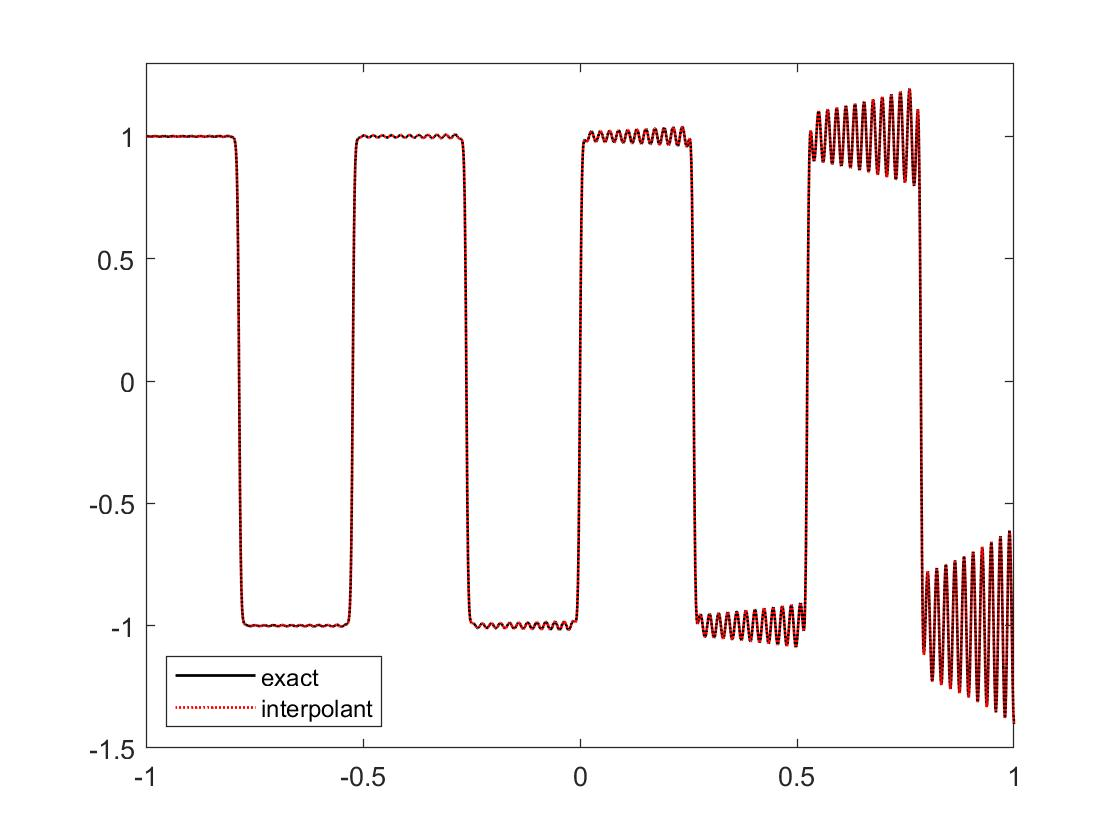
\includegraphics[width = .8\textwidth]{1.d.interpolant.jpg}

误差:\\
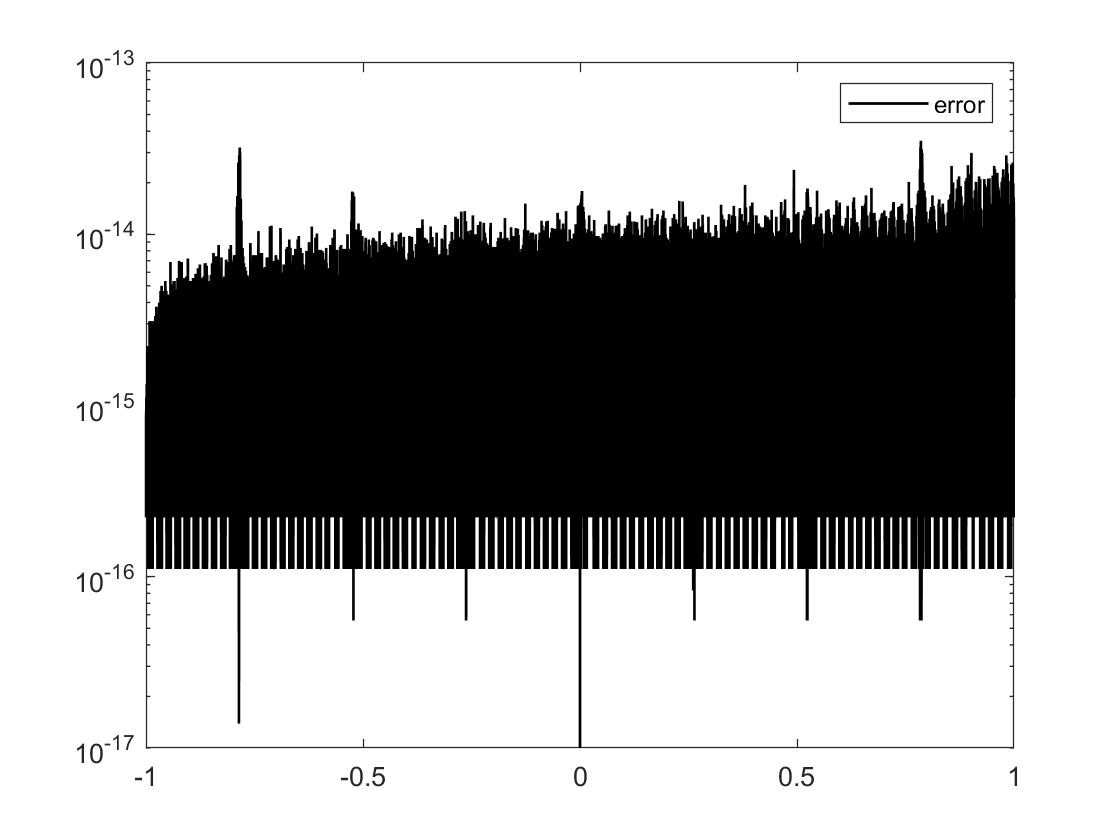
\includegraphics[width = .8\textwidth]{1.d.error.jpg}

\item[第二题]
\textsc{Matlab}程序如下:
\begin{lstlisting}[frame=single]
clear, clc, clf
LW = 'linewidth'; lw = 2;
MaxError1 = zeros(7, 1);
MaxError2 = zeros(7, 1);
MaxError3 = zeros(7, 1);
for k = 6:12
    %%
    n = 2 ^ k;
    x = linspace(-n, n, n+1)' ./ n;
    F = @(x)exp(3*cos(pi*x));
    DF = @(x)-3*pi*exp(3*cos(pi*x)).*sin(pi*x);
    D2F = @(x)9*pi^2*exp(3*cos(pi*x)).*sin(pi*x).^2 - ...
        3*pi^2*exp(3*cos(pi*x)).*cos(pi*x);
    f = F(x);
    Df = DF(x);
    D2f = D2F(x);
    %%
    h = diff(x);
    df = diff(f);
    d1 = df ./ h;
    lambda = h(2:n) ./ (h(2:n) + h(1:n-1));
    d = 6 * (df(2:n)./h(2:n) - df(1:n-1)./h(1:n-1)) ./ ...
        (h(2:n) + h(1:n-1));
    mu = 1-lambda;
    %%
    % 第一类边界条件
    M0 = D2f(1);
    Mn = D2f(n + 1);
    A1 = diag(2*ones(n-1,1)) + diag(lambda(1:n-2), 1) +...
        diag(mu(2:n-1), -1);
    D1 = [d(1)-mu(1)*M0; d(2:n-2); d(n-1)-lambda(n-1)*Mn];
    M1 = A1 \ D1;
    M1 = [M0; M1; Mn];
    %%
    % 第二类边界条件
    m0 = Df(1);
    mn = Df(n + 1);
    lambda2 = [1; lambda];
    mu2 = [mu; 1];
    d0 = 6 * ( df(1) / h(1) - m0 ) / h(1);
    dn = 6 * ( mn - df(n) / h(n) ) / h(n);
    D2 = [d0; d; dn];
    A2 = diag(2*ones(n+1,1))+diag(lambda2,1)+diag(mu2,-1);
    M2 = A2 \ D2;
    %%
    % 第三类边界条件
    lambda0 = h(1) / (h(1) + h(n));
    lambda3 = [lambda0; lambda(1:n-2)];
    mu0 = 1 - lambda0;
    d0 = 6*(df(1)./h(1) - df(n)./h(n)) / (h(1)+h(n));
    D3 = [d0; d];
    A3 = diag(2*ones(n,1)) + diag(lambda3,1) +diag(mu,-1);
    A3(1, n) = mu0;
    A3(n, 1) = lambda(n-1);
    M3 = A3 \ D3;
    M3 = [M3; M3(1)];
    %%
    MaxError1(k - 5) = CubicSpline(x, F, h, M1);
    MaxError2(k - 5) = CubicSpline(x, F, h, M2);
    MaxError3(k - 5) = CubicSpline(x, F, h, M3);
end
%%
xx = linspace(6, 12, 7);
semilogy(xx, MaxError1, 'r:', LW, lw), hold on
semilogy(xx, MaxError2, 'gx', LW, lw), hold on
semilogy(xx, MaxError3, 'b')
legend('第一类', '第二类', '第三类')
%%
function MaxError = CubicSpline(x, F, h, M)
n = size(x) - 1;
f = F(x);
MaxError = 0;
for k = 1:n
    m = 6;
    xx = linspace(x(k), x(k+1), m)';
    S = ((x(k+1)-xx).^3*M(k) + (xx-x(k)).^3*M(k+1)) / ...
        (6*h(k)) + ...
        ((x(k+1)-xx)*f(k) + (xx-x(k))*f(k+1)) / h(k) - ...
        h(k) * ((x(k+1)-xx)*M(k) + (xx-x(k))*M(k+1)) / 6;
    MaxError = max([MaxError, abs(F(xx) - S)']);
end
end
\end{lstlisting}

最大误差:\\
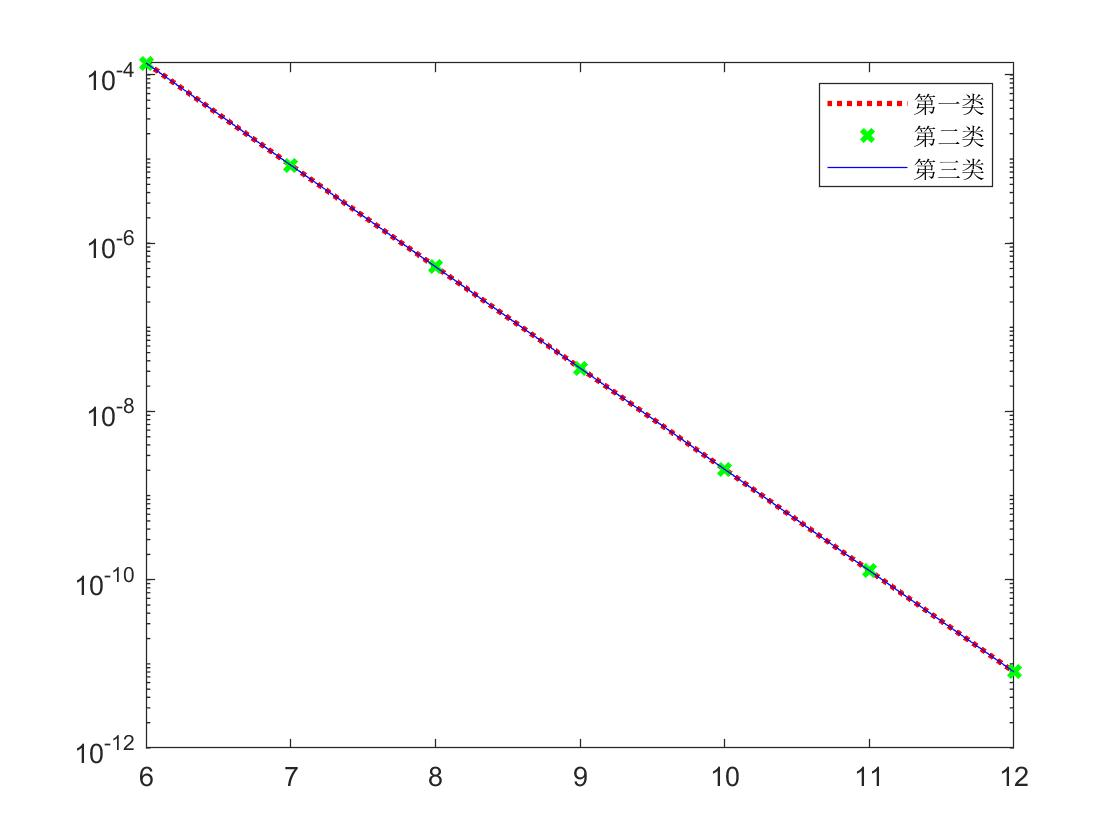
\includegraphics[width = .8\textwidth]{2.jpg}

\item[第三题]
\textsc{Matlab}程序如下:
\begin{lstlisting}[frame=single]
x = [-0.7, -0.5, 0.25, 0.75];
y = [0.99, 1.21, 2.57, 4.23];
% y=a*exp(bx)
% lny=bx+lna
lny = log(y);
R = [x' ones(4, 1)];
% solve A
A = R \ lny';

a = exp(A(2));
b = A(1);
F = @(x)a*exp(b*x);
f = F(x);
% error
M2 = sqrt((y - f) * (y - f)')

xx = linspace(-1, 1, 1000);
plot(xx, F(xx), 'k', x, y, 'x')
\end{lstlisting}

拟合函数图像:\\
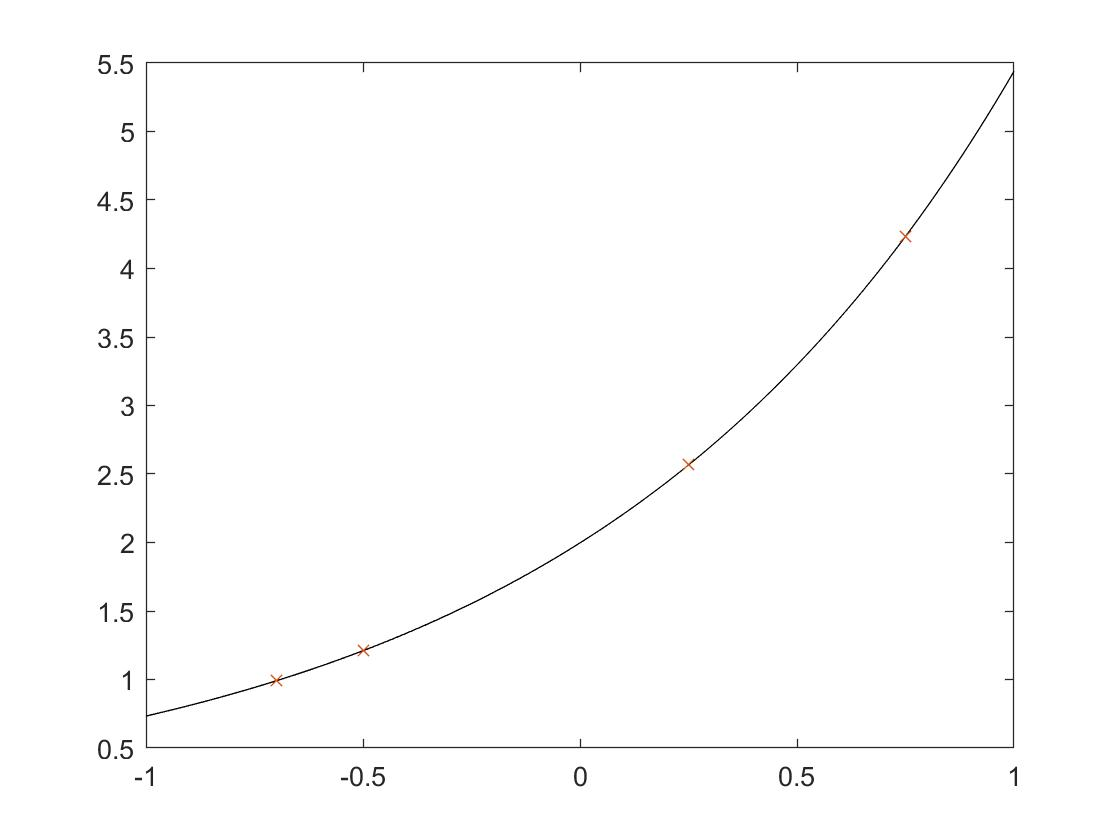
\includegraphics[width = .8\textwidth]{3.jpg}

误差的2-范数为$0.0062$.
\end{enumerate}

\end{document}
